\section{Introduction to GUI (a)}

When the application first starts the user has the option to select either their own
map, or a map that has been included by default. If the user wants to load their own map, they should selected
user generated map and input the file path into the file input text field. Otherwise, they
can simply select a pre-generated map from the drop down menu along with its variation.

There are a total of 4 algorithms included in the main menu that the user can then select from to find a path
from the start to goal. Options include: Uniform cost search, A*, Weighted A*, and Sequential A*. If the
user selects weighted or sequential A* they should input two weights into the weight text fields. Once all the parameters
are selected by the user, they can select confirm and the map along with its solution using the selected algorithm
will be loaded.


\begin{figure}[H]
	\centering
%  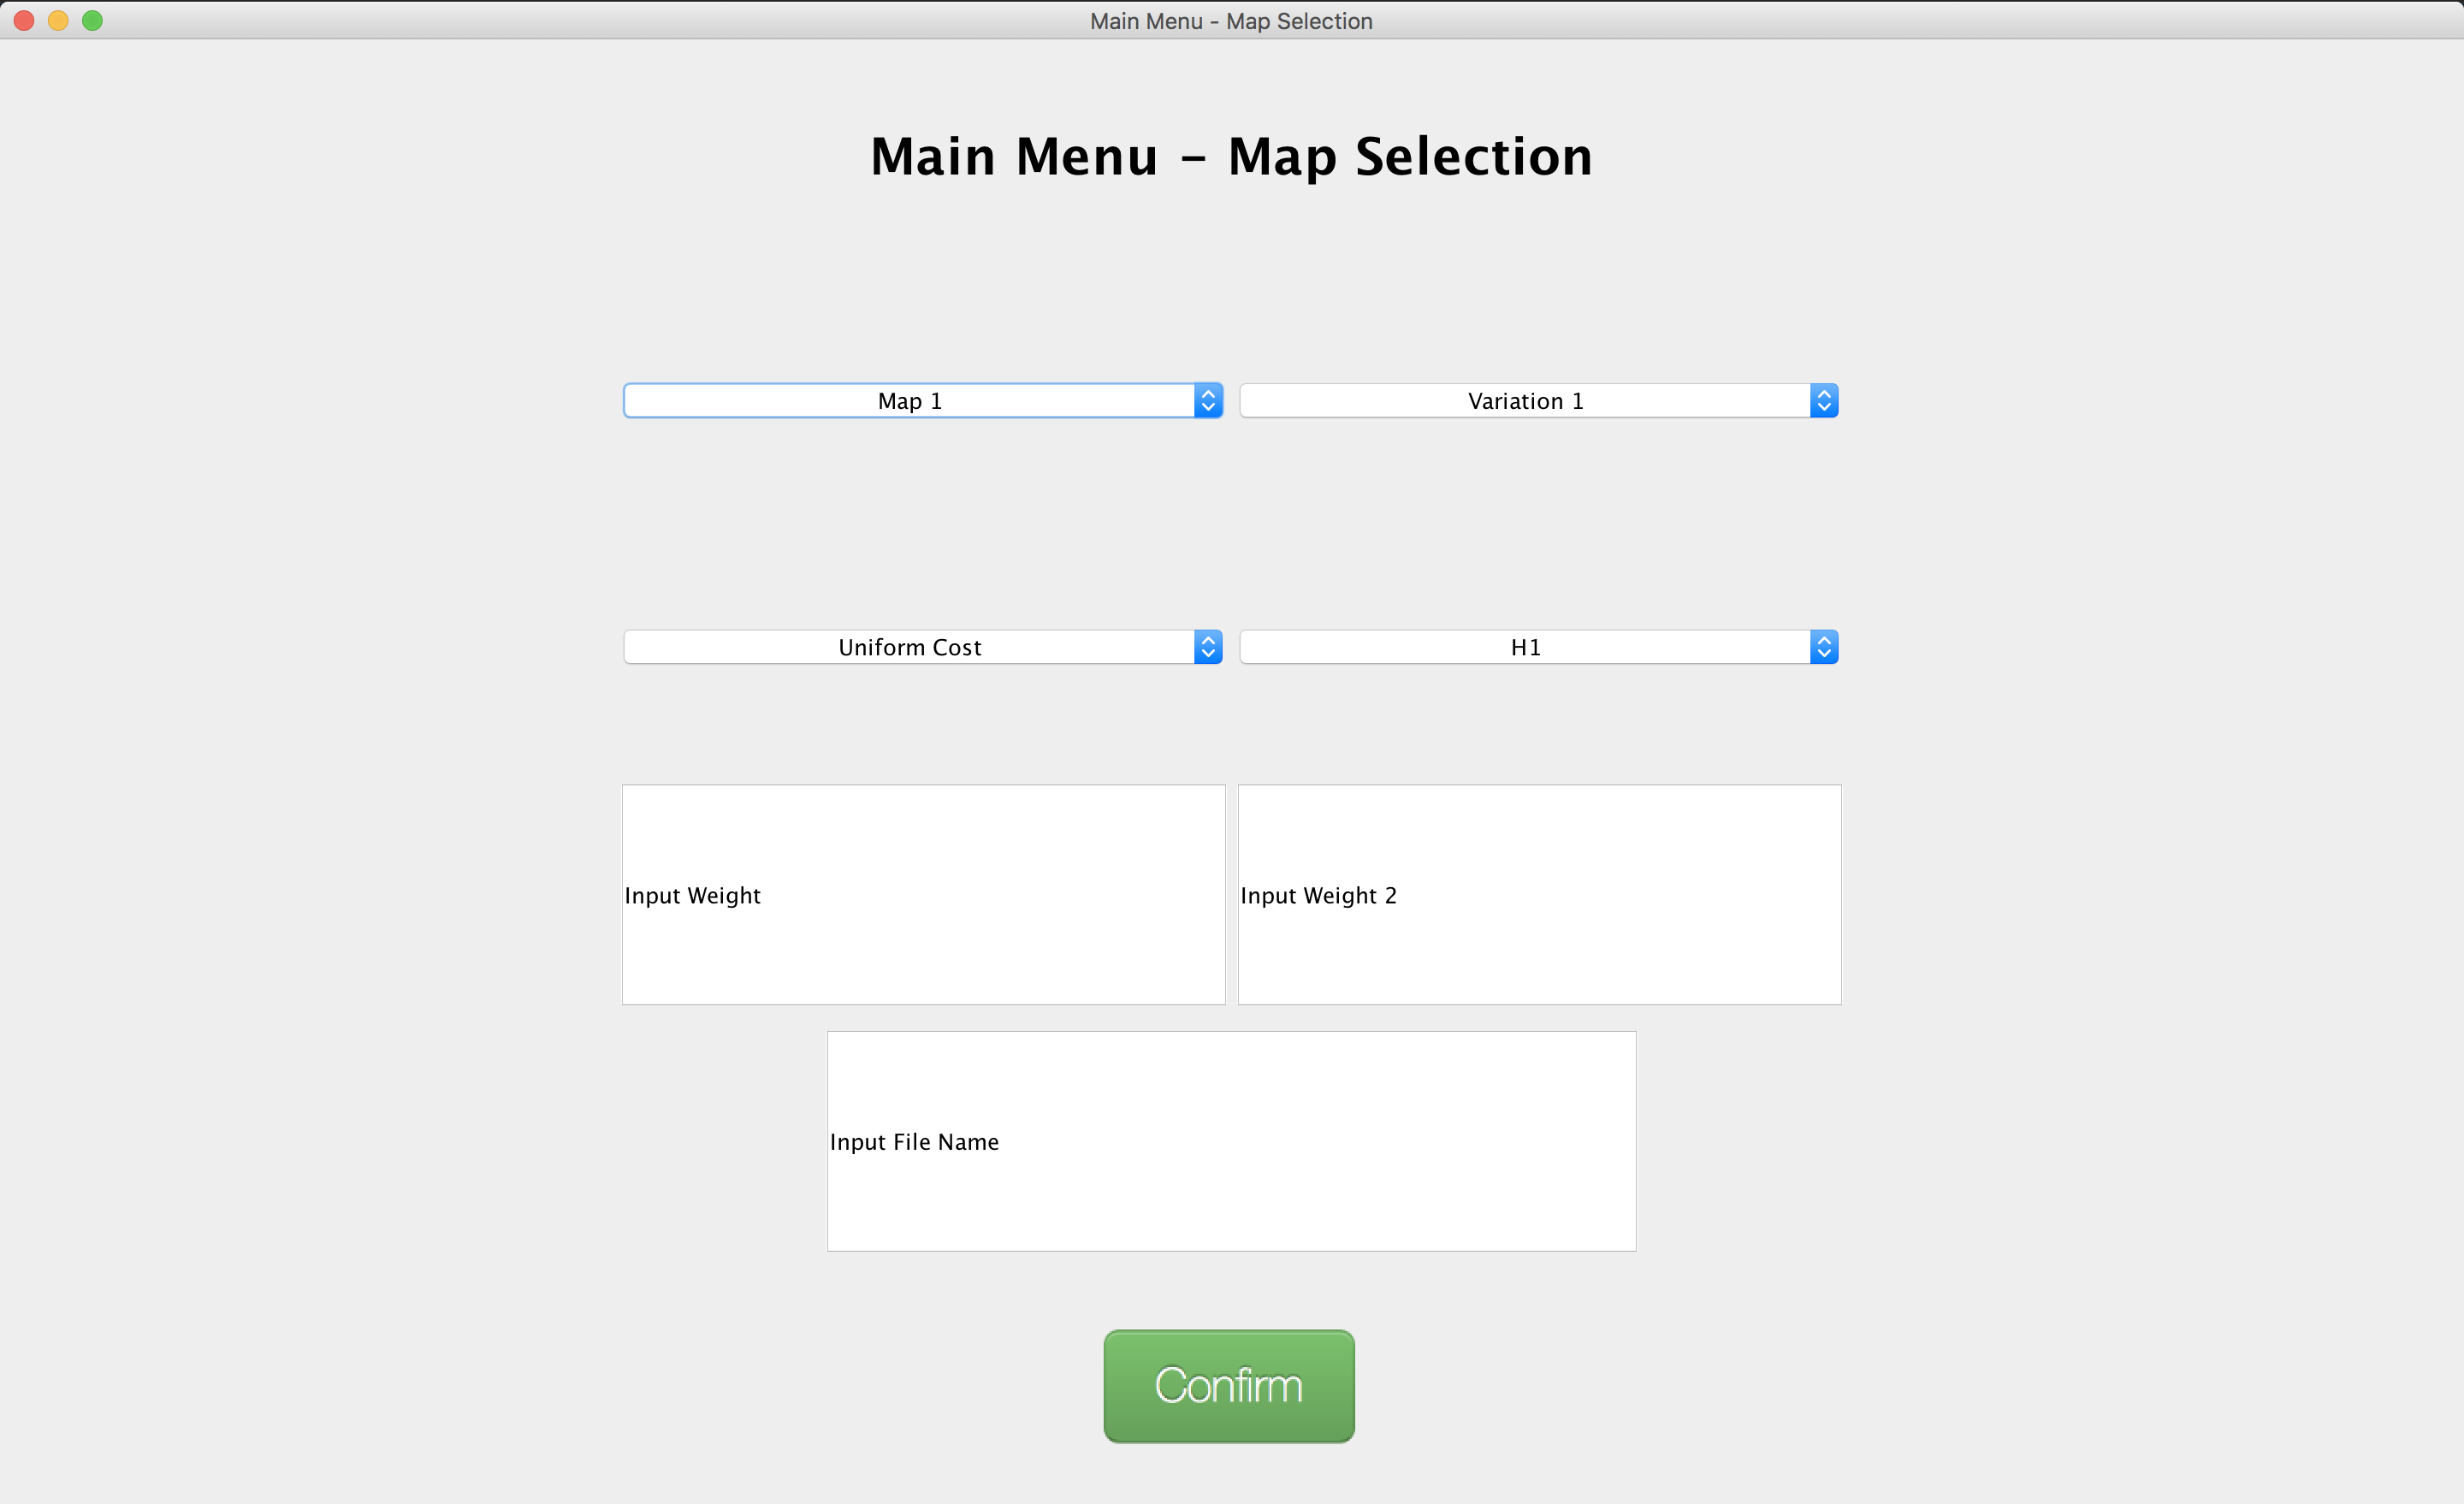
\includegraphics[scale = 0.30]{main_menu.png}
	\caption{The main menu of the application}
	\label{fig: Main menu}
\end{figure}
